% Compile with XeLaTeX in the Codex LaTeX editor.
\documentclass[12pt,a4paper]{report}
\usepackage[a4paper,margin=2.5cm]{geometry}
\usepackage{fontspec}
\setmainfont{Times New Roman}
\usepackage{polyglossia}
\setdefaultlanguage{vietnamese}
\usepackage{amsmath,amssymb,booktabs,longtable,graphicx,hyperref,xcolor,listings,enumitem}
\usepackage{setspace}
\usepackage[numbers,sort&compress]{natbib}
\hypersetup{colorlinks=true,linkcolor=blue,citecolor=blue,urlcolor=blue}
\lstset{basicstyle=\ttfamily\small,breaklines=true,frame=single}
\setlist{nosep,leftmargin=1.6em}
\setlength{\textfloatsep}{10pt plus 2pt minus 2pt}
\setlength{\floatsep}{8pt plus 2pt minus 2pt}
\setlength{\intextsep}{8pt plus 2pt minus 2pt}
\title{Phân đoạn từng đối tượng bằng Deep Learning với StarDist\\
\large Đối chiếu Fiji/ImageJ và cài đặt Python}
\author{Nhóm 03 -- Học viện Công nghệ Bưu chính Viễn thông\\
Thành viên: \underline{\hspace{10cm}}}
\date{Hạn nộp: 19/11}
\begin{document}
\setstretch{1.25}
\maketitle
\pagenumbering{roman}
\chapter*{Tóm tắt}
Phân đoạn từng đối tượng (instance segmentation) là bước nền tảng để đếm và đo
hình thái tế bào. Báo cáo nghiên cứu StarDist 2D, một phương pháp dùng mạng
CNN để dự đoán xác suất tâm đối tượng và khoảng cách theo các tia, sau đó giải
mã đa giác star-convex và loại proposal trùng bằng Non-Maximum Suppression
(NMS). Nhóm xây dựng pipeline Python tái lập được, tự cài đặt các thao tác hình
học và đánh giá instance, đồng thời dùng plugin StarDist của Fiji/ImageJ làm
nền tảng tham chiếu. Otsu và marker-controlled Watershed là hai baseline. Kết
quả cuối được đánh giá bằng matching một-một theo IoU, AP tại nhiều ngưỡng,
Panoptic Quality, Dice foreground, sai số đếm và thời gian xử lý. Các label TIFF
Fiji/ImageJ, log tham số và metric của ba ca kiểm chứng được lưu cùng mã nguồn.

\chapter*{Từ khóa} StarDist, instance segmentation, U-Net, star-convex, Fiji,
ImageJ, Otsu, Watershed, Panoptic Quality.
\tableofcontents
\clearpage\pagenumbering{arabic}

\chapter{Giới thiệu}
\section{Bối cảnh và động cơ}
Ảnh hiển vi thường chứa nhiều nhân tế bào sát nhau. Mask foreground nhị phân
chỉ trả lời pixel nào thuộc tế bào, nhưng không trả lời pixel đó thuộc tế bào
nào. Vì vậy, một vùng chạm nhau có thể bị gộp thành một object, làm sai số đếm,
diện tích và các phép đo hình thái. Instance segmentation yêu cầu một nhãn
riêng cho từng object, khác semantic segmentation và object detection chỉ dùng
bounding box.

StarDist biểu diễn mỗi object bằng một đa giác star-convex, phù hợp với nhiều
nhân tế bào dạng blob. So với cách phân đoạn bottom-up, các proposal hình học
và NMS giúp tách object ngay cả khi ranh giới pixel mờ \citep{schmidt2018stardist}.
Tuy nhiên giả thiết star-convex không phù hợp hoàn toàn với object hình vòng,
phân nhánh hoặc lõm sâu; đánh giá trên dữ liệu mục tiêu là bắt buộc.

\section{Mục tiêu và đóng góp}
Mục tiêu là nghiên cứu, cài đặt, thực nghiệm và đánh giá StarDist 2D với Fiji
làm tham chiếu. Sản phẩm gồm: (i) mô hình toán học của StarDist, CNN/U-Net,
Otsu và Watershed; (ii) protocol Fiji có log tham số và macro batch; (iii)
package Python với CLI, baseline, geometry reference và metric; (iv) thiết kế
thí nghiệm định lượng; và (v) báo cáo, presentation.

\section{Câu hỏi nghiên cứu}
RQ1 kiểm tra StarDist có tách object chạm nhau tốt hơn Otsu/Watershed không.
RQ2 kiểm tra tính tương thích Fiji--Python khi giữ nguyên input và tham số.
RQ3 đo độ nhạy của probability threshold và NMS threshold. Mỗi câu hỏi dùng
test set cố định; validation chỉ dùng để chọn tham số.

\chapter{Cơ sở lý thuyết}
\section{Bài toán instance segmentation}
Cho ảnh $I:\Omega\rightarrow\mathbb{R}^C$, với miền pixel
$\Omega=\{0,\ldots,H-1\}\times\{0,\ldots,W-1\}$ và $C$ kênh. Ground truth
là ảnh nhãn nguyên $Y:\Omega\rightarrow\{0,1,\ldots,M\}$: $Y(q)=0$ là nền;
mọi pixel mang cùng nhãn $m>0$ tạo thành instance $G_m$. Mục tiêu là ước lượng
$\hat Y=f_\theta(I)$ sao cho từng object có ID riêng, kể cả khi hai object cùng
lớp chạm biên. Đây là khác biệt cốt lõi giữa ba nhiệm vụ thường bị nhầm lẫn:

\begin{itemize}
\item \textbf{Semantic segmentation} dự đoán foreground/background hoặc lớp tại
mỗi pixel; hai nhân chạm nhau vẫn có thể là một vùng liên thông.
\item \textbf{Object detection} trả bounding box và score, hữu ích để định vị
nhưng không đủ cho diện tích, chu vi hay hình dạng nhân.
\item \textbf{Instance segmentation} trả tập mask/polygon $\{P_j\}_{j=1}^N$;
các $P_j$ được phân biệt theo ID và là đầu vào đúng cho phép đếm.
\end{itemize}

Trong ảnh hiển vi, sai khác giữa foreground mask và instance label có ảnh hưởng
trực tiếp đến định lượng: hai nhân dính nhau làm số object giảm một, diện tích
tăng giả tạo và các đặc trưng hình thái bị trộn. Vì vậy, một Dice foreground
cao chưa bảo đảm chất lượng instance; báo cáo cần matching theo từng object ở
nhiều ngưỡng IoU.

\subsection{Tiền xử lý và quy ước số học}
Các model pretrained nhạy với thang cường độ. Với percentile thấp/cao $a,b$,
chuẩn hoá dùng trong thí nghiệm là
\begin{equation}
 I_{\mathrm{norm}}(q)=\operatorname{clip}\left(
 \frac{I(q)-Q_a(I)}{Q_b(I)-Q_a(I)+\varepsilon},0,1\right),
 \label{eq:percentile-normalization}
\end{equation}
trong đó $Q_a,Q_b$ là percentile và $\varepsilon$ tránh chia cho 0. Nó không
thay đổi toạ độ hay pixel size, nhưng giới hạn ảnh hưởng của outlier sáng/tối.
Trong cả Fiji và Python, cùng $a=1$, $b=99.8$ được giữ cố định. Label output
luôn là TIFF 2D số nguyên, không phải ảnh RGB màu; màu chỉ dùng để hiển thị ID.

\section{CNN và U-Net}
\subsection{Tích chập, receptive field và phi tuyến}
CNN học các kernel thay vì thiết kế thủ công feature. Với feature map đầu vào
$a^{(l-1)}$ và kernel $w^{(l)}$, giá trị ở lớp $l$ là
\begin{equation}
 a_{i,j,c}^{(l)}=\phi\left(b_c^{(l)}+\sum_{u,v,c'}w_{u,v,c',c}^{(l)}
 a_{i+u,j+v,c'}^{(l-1)}\right).
 \label{eq:convolution}
\end{equation}
Hàm phi tuyến $\phi$ (ví dụ ReLU) cho phép xấp xỉ quan hệ phi tuyến giữa cấu
trúc ảnh và nhãn. Khi nhiều lớp và pooling/strided convolution nối tiếp, một
pixel đầu ra quan sát được vùng lân cận lớn hơn, gọi là \emph{receptive field}.
Ngữ cảnh này hữu ích để phân biệt đốm nhiễu với nhân tế bào, nhưng downsampling
quá mạnh sẽ làm mất chi tiết biên.

\subsection{U-Net làm backbone đa đầu ra}
U-Net gồm encoder giảm dần độ phân giải để học ngữ cảnh, bottleneck, rồi decoder
upsampling để khôi phục lưới pixel. Skip connection nối feature map cùng scale
từ encoder sang decoder, giúp decoder dùng lại vị trí/biên mảnh thay vì chỉ dựa
vào feature đã nén \citep{ronneberger2015unet}. StarDist dùng U-Net như backbone
chia sẻ và gắn hai head $1\times1$ convolution tại độ phân giải ảnh:
\begin{equation}
 (\hat p(q),\hat{\mathbf r}(q))=h_\theta(I)(q),\qquad
 \hat p(q)\in[0,1],\quad \hat{\mathbf r}(q)\in\mathbb{R}_+^K.
 \label{eq:stardist-heads}
\end{equation}
Head probability trả một kênh score; head hình học trả $K$ khoảng cách tia.
Vì hai task dùng cùng feature, score có thể đánh giá độ tin cậy proposal còn
distance head mô tả biên object. Mạng \emph{không} sinh trực tiếp một label ID
cho mỗi pixel, vì ID không có thứ tự cố định giữa các ảnh.

\section{Probability map và star-convex polygon}
\subsection{Giả thiết star-convex và target radial distance}
Một tập $S$ là star-convex đối với điểm $c$ nếu mọi đoạn thẳng từ $c$ đến điểm
$x\in S$ đều nằm trong $S$, tức $[c,x]\subseteq S$. Đối với một pixel
foreground $q$ và $K$ hướng đều nhau $\theta_k=2\pi k/K$, target radial là
\begin{equation}
 r_k(q)=\max\{t\ge0:q+t(\cos\theta_k,\sin\theta_k)\in G(q)\},
 \quad k=0,\ldots,K-1,
 \label{eq:ray-distance}
\end{equation}
trong đó $G(q)$ là instance chứa $q$. Nói cách khác, ta đi từ $q$ theo từng tia
đến giao điểm đầu tiên với biên. Bài báo gốc dùng $K=32$ \citep{schmidt2018stardist};
$K$ lớn hơn mô tả biên cong tốt hơn nhưng tăng số kênh, bộ nhớ và số polygon
phải xử lý trong NMS.

Khi mạng dự đoán $\hat{\mathbf r}(q)$, các đỉnh polygon proposal là
\begin{equation}
 v_k(q)=q+\hat r_k(q)(\cos\theta_k,\sin\theta_k).
 \label{eq:polygon-vertices}
\end{equation}
Nối $v_0,\ldots,v_{K-1}$ theo thứ tự góc tạo polygon xấp xỉ instance. Một object
có thể sinh proposal từ nhiều pixel bên trong nó, nhưng proposal gần tâm thường
ổn định hơn. Target probability $p(q)$ là Euclidean distance transform (EDT)
chuẩn hoá riêng trong từng instance: gần biên có giá trị xấp xỉ 0, trung tâm có
giá trị cao. Do đó probability map vừa là foreground confidence vừa thiên về
những tâm sinh polygon tốt.

\subsection{Khả năng biểu diễn và giới hạn}
Star-convex polygon phù hợp nhân tế bào/bào quan dạng khối tròn hoặc bầu dục,
và tách hai nhân sát nhau bằng hai polygon chồng cạnh. Ngược lại, hình vòng,
nhánh cây hoặc lõm sâu có thể không nhìn thấy toàn bộ biên từ một tâm; ray đi
qua nền rồi vào lại object làm biểu diễn không đúng. Lỗi khi đó là hạn chế mô
hình hình học, không chỉ là lỗi threshold. Cần kiểm tra overlay và cân nhắc
Watershed, Mask R-CNN hay fine-tuning đối với dữ liệu có hình dạng này.

\section{Huấn luyện và NMS}
\subsection{Hàm mất mát đa nhiệm}
Mạng học probability $\hat p$ và vector distance $\hat{\mathbf r}$. Với target
$p,\mathbf r$, một dạng objective điển hình là
\begin{align}
 \mathcal{L}_{\mathrm{prob}}&=-\frac1{|\Omega|}\sum_{q\in\Omega}
 [p(q)\log\hat p(q)+(1-p(q))\log(1-\hat p(q))],\\
 \mathcal{L}_{\mathrm{dist}}&=\frac{\sum_q p(q)\,\|\mathbf r(q)-
 \hat{\mathbf r}(q)\|_1}{\sum_q p(q)+\varepsilon},\\
 \mathcal{L}&=\lambda_p\mathcal{L}_{\mathrm{prob}}+
 \lambda_r\mathcal{L}_{\mathrm{dist}}.
 \label{eq:stardist-loss}
\end{align}
Trọng số $p(q)$ giảm tác động của pixel biên, nơi tia ngắn và nhạy với
annotation, đồng thời nhấn vào các tâm. Khi dùng pretrained model, các trọng
số đã được học trước; thí nghiệm này chỉ làm inference, không tuyên bố train
lại CNN.

\subsection{Suy luận, candidate filtering và polygon NMS}
Tại inference, tạo candidate $C=\{q:\hat p(q)\ge t_p\}$. Mỗi $q\in C$ được
decode theo~\eqref{eq:polygon-vertices}; sau đó sắp giảm dần theo $\hat p(q)$.
Với proposal được giữ $A$ và proposal xét $B$, overlap là
\begin{equation}
 \operatorname{IoU}(A,B)=\frac{|A\cap B|}{|A\cup B|}.
 \label{eq:polygon-iou}
\end{equation}
NMS giữ proposal score cao nhất còn lại và loại mọi proposal có
$\operatorname{IoU}(A,B)>t_{\mathrm{nms}}$; lặp đến khi hết candidate. Các
polygon được giữ được raster hoá thành label ID không chồng nhau. Độ phức tạp
CNN gần tuyến tính theo số pixel, còn hậu xử lý phụ thuộc số candidate và cặp
polygon; vì vậy $t_p$, tile size và NMS ảnh hưởng runtime.

Hai threshold có ý nghĩa khác nhau, cần ghi tách biệt trong log. $t_p$ thấp quá
tạo nhiều positive giả và tăng chi phí NMS; cao quá làm mất object mờ. Ngưỡng
$t_{\mathrm{nms}}$ thấp triệt proposal mạnh (dễ bỏ sót object sát nhau); cao
dễ giữ trùng lặp. Các giá trị thực tế ở đây là $t_p=0.479071$ và
$t_{\mathrm{nms}}=0.3$, được lấy từ cấu hình model, không tune trên test.

\section{Baseline Otsu và Watershed}
\subsection{Otsu và connected components}
Otsu giả định histogram có thể tách thành hai lớp bằng ngưỡng $t$. Gọi
$\omega_0,\omega_1$ là xác suất hai lớp và $\mu_0,\mu_1$ là trung bình cường
độ của chúng, Otsu chọn
\begin{equation}
 t^*=\arg\max_t\;\sigma_B^2(t),\qquad
 \sigma_B^2(t)=\omega_0(t)\omega_1(t)[\mu_0(t)-\mu_1(t)]^2.
 \label{eq:otsu}
\end{equation}
Sau threshold, lọc vùng nhỏ và connected components 8-neighbour tạo label.
Điểm mạnh là không cần model, nhanh và có thể giải thích; điểm yếu là nền không
đồng nhất/ảnh ít tương phản làm histogram không còn bimodal. Quan trọng hơn,
hai object chạm nhau thành một component nên Otsu thường có Dice foreground tốt
nhưng AP instance và count kém.

\subsection{Marker-controlled Watershed}
Watershed bổ sung bước tách object trên foreground mask $F$. Đầu tiên tính
$D=\operatorname{EDT}(F)$; đỉnh địa phương của $D$ là marker gần tâm object.
Thuật toán ``ngập'' landscape $-D$ từ các marker và đặt watershed line nơi hai
vùng gặp nhau \citep{vincent1991watersheds}. Pipeline triển khai là: (1) Otsu
tạo $F$; (2) morphology/loại vùng nhỏ; (3) peak-local-max với khoảng cách tối
thiểu $d$; (4) watershed của $-D$ bị ràng buộc trong $F$; (5) relabel output.
Nó tách được nhân tiếp xúc tốt hơn Otsu nhưng over-segment khi marker nhiễu,
under-segment khi hai đỉnh quá gần hoặc một nhân không có cực đại rõ. Vì vậy
$d$ phải chọn trên validation thay vì test.

\subsection{So sánh khái niệm}
Otsu và Watershed là phương pháp bottom-up dựa trên cường độ/địa hình; StarDist
là phương pháp learned proposal có prior star-convex. Baseline không cạnh tranh
công bằng về lượng thông tin học được, nhưng cần thiết để xác định mức cải thiện
thực sự so với xử lý ảnh cổ điển. Cả ba xuất cùng chuẩn label TIFF và đi qua
cùng metric, do đó so sánh không bị ảnh hưởng bởi cách hiển thị màu.

\chapter{Fiji/ImageJ làm nền tảng tham chiếu}
\section{Plugin StarDist}
Plugin StarDist của Fiji cung cấp inference cho model 2D pretrained/custom,
percentile normalization, probability threshold, overlap/NMS threshold, tile
và output label image/ROI \citep{imagej_stardist_plugin}. Fiji là công cụ tham
chiếu cho thao tác trực quan và đo đạc, không thay thế đánh giá định lượng.

\subsection{Vai trò của ImageJ, Fiji và plugin}
ImageJ là nền tảng xử lý ảnh có ImagePlus, ROI Manager, macro recorder và hệ
sinh thái plugin. Fiji là bản phân phối ImageJ đã tích hợp nhiều plugin khoa
học và cơ chế update site; StarDist là plugin inference chạy trong runtime đó.
Vì vậy, ``mở bằng Fiji'' không tự động bảo đảm tái lập: phải ghi phiên bản
plugin, model, Java/TensorFlow, input, chuẩn hoá, threshold, tile và kiểu output.
Trong báo cáo này, output chuẩn để đối chiếu là \textbf{Label Image TIFF}: nền
có ID 0 và mỗi instance có ID nguyên dương. ROI Manager chỉ phục vụ quan sát,
không dùng thay label để tính metric.

\subsection{Thông số có ý nghĩa thực nghiệm}
\begin{longtable}{p{3.2cm}p{4.0cm}p{6.2cm}}
\toprule
Tham số & Giá trị lần chạy tham chiếu & Ý nghĩa/điểm cần kiểm tra\\
\midrule\endfirsthead
\toprule Tham số & Giá trị lần chạy tham chiếu & Ý nghĩa/điểm cần kiểm tra\\\midrule\endhead
Model & Versatile (fluorescent nuclei) & Phải phù hợp modality; không dùng model H\&E cho ảnh huỳnh quang.\\
Normalize & percentile 1 / 99.8 & Cùng công thức~\eqref{eq:percentile-normalization} ở Fiji và Python.\\
Probability threshold & 0.479071 & Lọc candidate trước NMS; không tối ưu lại trên ba ảnh kiểm chứng.\\
NMS overlap & 0.3 & Khử proposal polygon trùng; khác với IoU threshold khi đánh giá.\\
Tiles / exclude boundary & 1 / 2 px & Tile ảnh hưởng bộ nhớ và seam; boundary exclusion thay đổi object nằm sát biên.\\
Output & Label Image TIFF & Phải cùng kích thước với input/ground truth; không lưu PNG RGB để đo.\\
\bottomrule
\end{longtable}

\section{Protocol tái lập và lần chạy thực tế}
Ngoài protocol GUI, nhóm chạy command StarDist đã công bố
\texttt{de.csbdresden:StarDist\_:0.3.0-scijava} trong ImageJ 2.9.0 headless,
với ImageJ 1.53t legacy, Eclipse Temurin 8.0.504 và TensorFlow 1.12 CPU. Đây là
chính artifact plugin dùng cho Fiji/ImageJ; Java~8 cần thiết vì TensorFlow
ImageJ 1.12 là runtime cũ. Ba ảnh low/median/high được chọn trước từ test split
theo AP của StarDist Python, không tune threshold trên ba ảnh này. Model là
\emph{Versatile (fluorescent nuclei)}, percentile $1/99.8$, probability
$0.479071$, overlap/NMS $0.3$, một tile và boundary exclusion~2. Plugin xuất
Label Image TIFF cùng kích thước input. Mỗi lần chạy và runtime được ghi trong
\texttt{fiji/run\_log\_dsb2018\_reference.csv}; runner Java là
\texttt{fiji/scripts/FijiStarDistRunner.java}.

File \texttt{fiji/workflows/stardist\_fiji\_protocol.md} vẫn là hướng dẫn thao tác
Fiji GUI; macro \texttt{fiji/macros/stardist\_batch.ijm} yêu cầu dùng Fiji Recorder
để chèn đúng lệnh của phiên bản plugin, tránh đoán option macro.

\subsection{Các bước thao tác và bằng chứng cần lưu}
Quy trình GUI được áp dụng theo đúng thứ tự sau. Mỗi bước có artefact tương ứng
trong repository để người chấm kiểm tra thay vì chỉ tin vào mô tả.
\begin{enumerate}
\item Mở TIFF 2D và xác nhận kích thước/bit-depth/channel bằng
\texttt{Image > Show Info}. Lưu tên file input và không resize ảnh.
\item Mở \texttt{Plugins > StarDist > StarDist 2D}; chọn đúng model, nhập
percentile, probability, NMS, tile và bật \texttt{Label Image}.
\item Chạy inference; sau khi output xuất hiện, kiểm tra input và label cùng
chiều cao/rộng, quan sát overlay/ROI để phát hiện merge hoặc split bất thường.
\item Lưu label TIFF nguyên gốc; không export screenshot hay PNG để đánh giá.
Ghi runtime và tất cả parameter vào run log.
\item Chạy evaluator Python trên chính TIFF đó. Kiểm tra TP/FP/FN, overlay và
metric trước khi tổng hợp mean $\pm$ SD.
\end{enumerate}

Hình~\ref{fig:fiji-workflow} là bằng chứng trực quan của năm đầu ra từ workflow
thật ở ca median: TIFF input, input sau percentile normalization, label image,
overlay biên đối chiếu ground truth và block tham số/runtime trích từ run log.
Nó được dựng từ file đầu vào/đầu ra thực tế, không suy diễn label từ ảnh chụp.
Các output ba ca low/median/high đầy đủ tiếp tục được trình bày ở
Hình~\ref{fig:fiji-reference}.

\begin{figure}[htbp]
\centering
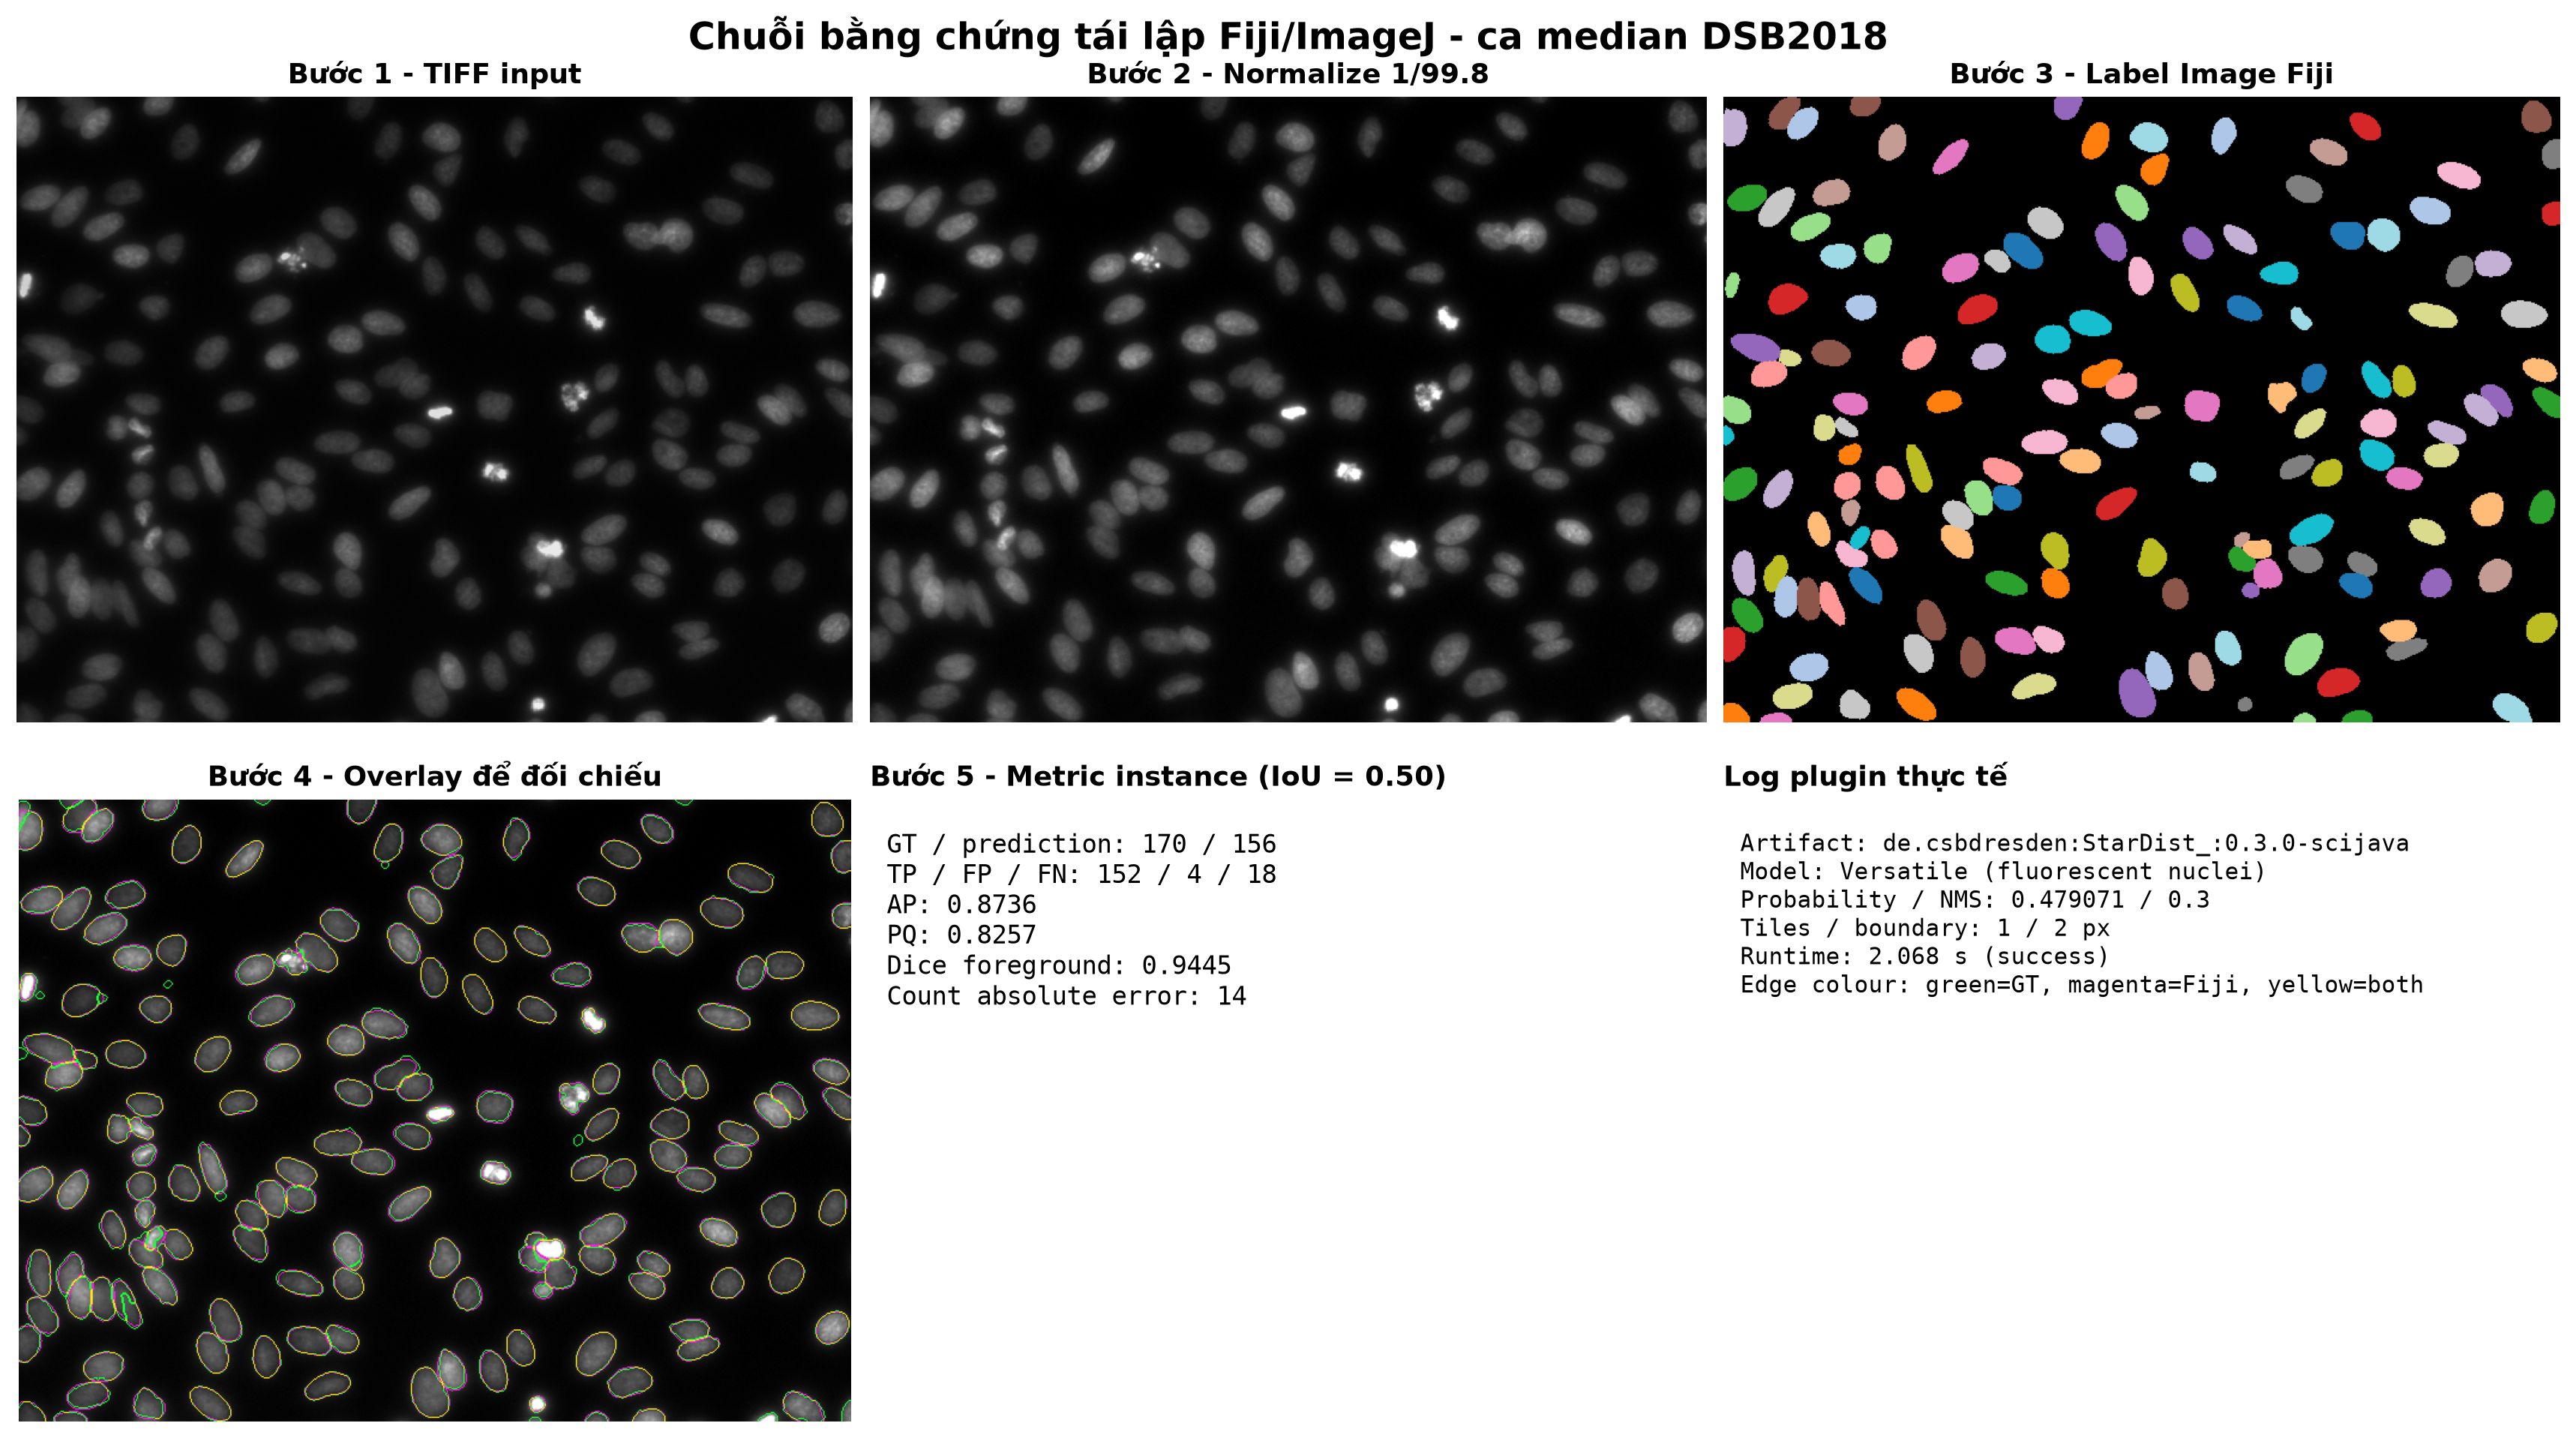
\includegraphics[width=\textwidth]{../results/fiji_reference/fiji_workflow_evidence.png}
\caption{Minh chứng từng bước của workflow Fiji/ImageJ trên ca median. Từ trái
sang phải: input TIFF, ảnh sau percentile 1/99.8, Label Image TIFF StarDist,
overlay prediction/ground truth và parameter/runtime thực tế. Đây là artefact
đầu ra của plugin/evaluator, không phải mask minh hoạ tự vẽ.}
\label{fig:fiji-workflow}
\end{figure}

\section{Kiểm chứng Fiji--Python}
Hai output chỉ được so sánh khi dùng cùng ảnh, model, scale, chuẩn hoá và hai
threshold. Python đọc trực tiếp label TIFF Fiji rồi ghép instance theo IoU.
Nếu số object khác nhau, kiểm tra overlay và run log trước, sau đó mới kết luận
do phiên bản/model hay hậu xử lý. Bảng dữ liệu cấp-ảnh nằm tại
\texttt{results/fiji\_reference/per\_image\_metrics.csv}; nó ghi cả TP, FP, FN,
Dice, PQ, sai số đếm, thời gian và ba threshold đánh giá. Do đó Fiji không chỉ
được quan sát bằng mắt mà được đặt vào cùng evaluator instance với Python.

\chapter{Cài đặt Python}
\section{Kiến trúc phần mềm}
Package \texttt{src/xla\_gr03} tách tiền xử lý, I/O TIFF, Otsu/Watershed, geometry,
StarDist wrapper, metrics và CLI. Mọi output là label integer 2D. Lệnh
`xla-gr03 segment` chạy một phương pháp; `xla-gr03 evaluate` xuất JSON metric.
Unit tests bao phủ geometry, metric, preprocessing, I/O và baseline.

\section{Phần nhóm tự cài đặt và phần tái sử dụng}
Nhóm tự cài đặt EDT chuẩn hoá theo instance, ray distance, polygon decode,
polygon NMS raster hoá, IoU matrix và Hungarian matching. CNN/model pretrained
được gọi từ thư viện StarDist chính thức \citep{stardist_repository}. Sự phân
biệt này tránh tuyên bố sai rằng nhóm tự train lại toàn bộ mạng.

\begin{lstlisting}[language=Python,caption={Ví dụ chạy một baseline}]
xla-gr03 segment data/raw/image_001.tif results/otsu_labels.tif \
  --method otsu --foreground bright --min-size 20
xla-gr03 evaluate data/ground_truth/image_001.tif results/otsu_labels.tif \
  --thresholds 0.5 0.75 0.9
\end{lstlisting}

\section{Tái lập môi trường}
Môi trường đề xuất dùng Python 3.11, NumPy, SciPy, scikit-image, tifffile,
pytest và ruff; extra `stardist` thêm TensorFlow, csbdeep và StarDist. Chạy
`conda env create -f environment.yml`, sau đó `pytest` và `ruff check .`.
Model weight và dữ liệu nội bộ/raw không được commit; ngoại lệ là bộ benchmark
DSB2018 đã giải nén (497 cặp TIFF, xấp xỉ 194 MiB) được versioned tại
\texttt{data/dsb2018/dsb2018/} để tái lập đúng kết quả báo cáo. Config mặc định
ở \texttt{configs/default.yaml}.

\chapter{Thiết kế thí nghiệm và metric}
\section{Dữ liệu và split}
Dataset phải có instance ground truth hợp pháp, ví dụ DSB2018 hoặc MoNuSeg.
Raw image và label TIFF cùng basename nằm trong `data/raw` và
\texttt{data/ground\_truth}. Development dùng để debug; validation chọn tham số; test
chỉ đánh giá cuối. Không tối ưu threshold trên test set.

\section{Matching và metric}
\label{sec:matching}
Gọi $G_i$ là instance ground truth thứ $i$ và $P_j$ là instance prediction thứ
$j$. Trước hết code bỏ nhãn nền 0, lập ma trận giao nhau pixel-wise rồi tính
\begin{equation}
 J_{ij}=\operatorname{IoU}(G_i,P_j)=\frac{|G_i\cap P_j|}{|G_i\cup P_j|}.
 \label{eq:instance-iou}
\end{equation}
Không được ghép một prediction với nhiều ground truth hoặc ngược lại, vì điều
đó có thể che giấu merge/split. Hungarian assignment tìm tập cặp một-một có
tổng IoU lớn; chỉ những cặp có $J_{ij}\ge\tau$ mới là TP. Ground truth chưa
ghép là FN, prediction chưa ghép là FP. Cách làm này phản ánh đúng lỗi tách
instance: một prediction gộp hai nhân chỉ có thể khớp tối đa một nhân và nhân
còn lại là FN.

Tại mỗi $\tau\in\{0.50,0.75,0.90\}$, các chỉ số là
\begin{align}
P&=TP/(TP+FP), & R&=TP/(TP+FN),\\
F1&=2TP/(2TP+FP+FN), & AP_\tau&=TP/(TP+FP+FN).
\end{align}
Ở đây $AP_\tau$ là tên metric theo benchmark StarDist/Data Science Bowl, không
phải area under precision--recall curve. $\tau=0.50$ trả lời ``có nhận đúng
object không'', còn $\tau=0.90$ đòi biên khớp rất chính xác. Bởi vậy, chỉ báo
cáo một ngưỡng có thể che mất lỗi hình dạng.

Panoptic Quality kết hợp nhận diện và chất lượng mask:
\begin{equation}
 PQ_\tau=\frac{\sum_{(i,j)\in\mathrm{TP}}J_{ij}}
 {TP+\tfrac12FP+\tfrac12FN}.
 \label{eq:pq}
\end{equation}
Tử số là segmentation quality trên các cặp khớp; mẫu số phạt lỗi detection.
Ngoài ra, foreground Dice
$2|F_G\cap F_P|/(|F_G|+|F_P|)$ và foreground IoU đo vùng nhân hợp nhất, nhưng
không phân biệt ID instance. Sai số đếm là $|N_P-N_G|$; runtime được đo per
image và ghi rõ có/không có tải model. Toàn bộ metric tính từng ảnh trước, rồi
báo cáo mean $\pm$ standard deviation trên đúng số ảnh của từng stratum.

\section{Protocol benchmark}
Otsu, Watershed và StarDist Python chạy trên toàn bộ 50 test images. Watershed
được chọn bằng validation; StarDist dùng default đã đóng gói. StarDist
Fiji/ImageJ chạy trên ba ca low/median/high cố định để kiểm chứng cross-platform
với output label thật, không được gộp vào ước lượng 50 ảnh. Báo cáo mean $\pm$
SD, số ảnh và runtime riêng cho từng stratum. Script
\texttt{scripts/run\_dsb2018\_benchmark.py} sinh benchmark 50 ảnh; script
\texttt{scripts/evaluate\_fiji\_reference.py} đọc Label Image Fiji rồi đo metric.

\chapter{Kết quả và thảo luận}
\section{Benchmark tái lập được trên DSB2018}
Nhóm chạy ba phương pháp trên 50 ảnh của test split trong archive DSB2018 do
StarDist công bố \citep{caicedo2019nucleus}. Ground truth là instance label
TIFF; không dùng binary mask. Watershed chọn `min\_distance` bằng sweep trên 30
ảnh lấy mẫu seed 42 từ 447 ảnh train, đạt AP@0.50 cao nhất tại giá trị 9. Các
50 ảnh test không tham gia chọn tham số. StarDist Python dùng model
\texttt{2D\_versatile\_fluo}, percentile $1/99.8$, default probability threshold
$0.479071$ và NMS threshold $0.3$ từ model. Runtime CPU không tính tải model
và warm-up. Lệnh benchmark Python sinh toàn bộ CSV, figure và provenance;
đường dẫn tái lập được liệt kê trong README và Phụ lục C.

\begin{longtable}{lrrrr}
\caption{Metric instance. Ba baseline/Python dùng 50 test images; Fiji/ImageJ dùng ba ca kiểm chứng cố định.}\label{tab:main}\\
\toprule
Method & AP@.50 & AP@.75 & AP@.90 & PQ@.50\\
\midrule\endfirsthead
\toprule Method & AP@.50 & AP@.75 & AP@.90 & PQ@.50\\\midrule\endhead
Otsu & $0.643\pm0.238$ & $0.453\pm0.276$ & $0.223\pm0.221$ & $0.627\pm0.208$\\
Watershed & $0.715\pm0.199$ & $0.501\pm0.266$ & $0.214\pm0.207$ & $0.677\pm0.166$\\
StarDist Fiji ($n=3$) & $0.801\pm0.244$ & $0.764\pm0.207$ & $0.406\pm0.324$ & $0.788\pm0.160$\\
StarDist Python & $0.853\pm0.120$ & $0.692\pm0.235$ & $0.305\pm0.313$ & $0.785\pm0.110$\\
\bottomrule
\end{longtable}

\clearpage

\begin{longtable}{lrrr}
\caption{Metric foreground, sai số đếm và runtime. Mỗi dòng Fiji là mean $\pm$ SD trên ba ca.}\label{tab:secondary}\\
\toprule
Method & Dice foreground & MAE count & Runtime (s/image)\\
\midrule\endfirsthead
\toprule Method & Dice foreground & MAE count & Runtime (s/image)\\\midrule\endhead
Otsu & $0.895\pm0.070$ & 14.06 & 0.0100\\
Watershed & $0.894\pm0.071$ & 6.94 & 0.0238\\
StarDist Fiji ($n=3$) & $0.950\pm0.017$ & $6.00\pm7.21$ & $1.420\pm0.590$\\
StarDist Python & $0.916\pm0.049$ & 3.44 & 0.1120\\
\bottomrule
\end{longtable}

\noindent\footnotesize\textit{Ghi chú về công bằng so sánh.} Dòng Fiji/ImageJ
là kiểm chứng triển khai trên ba ca đã cố định; không phải ước lượng chung cho
50 test images nên không dùng để xếp hạng trực tiếp với ba dòng $n=50$. Runtime
Fiji đo command CPU, bao gồm inference/model initialization của process Java;
runtime Python là inference sau warm-up.\normalsize

\begin{figure}[htbp]
\centering
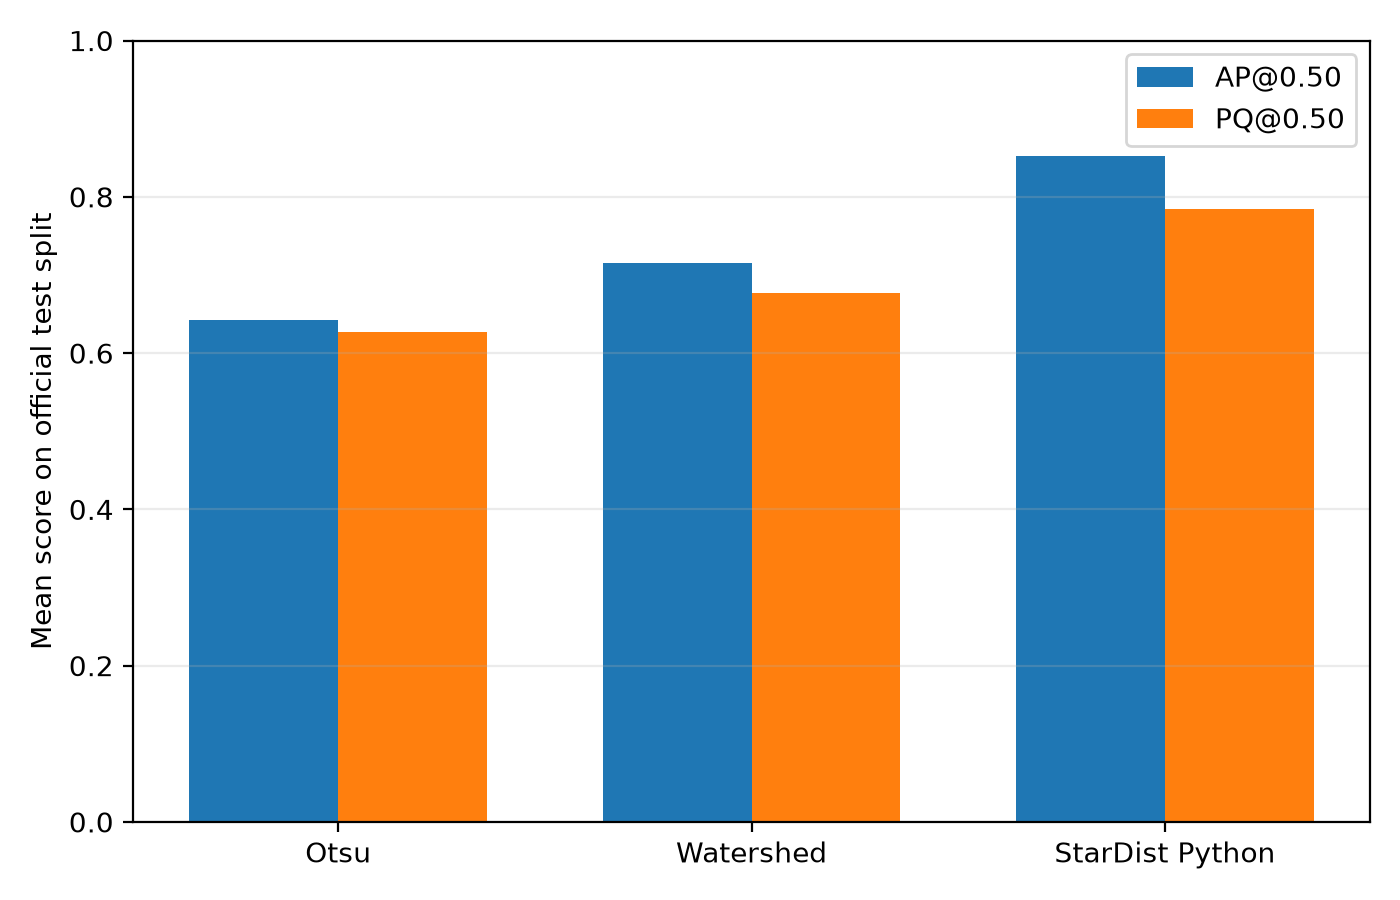
\includegraphics[width=.72\textwidth]{../results/dsb2018_benchmark/figures/benchmark_ap_pq.png}
\caption{Mean AP@0.50 và PQ@0.50 trên 50 ảnh test DSB2018. Error bar được
trình bày trong Bảng \ref{tab:main}.}
\label{fig:benchmark}
\end{figure}

\begin{figure}[htbp]
\centering
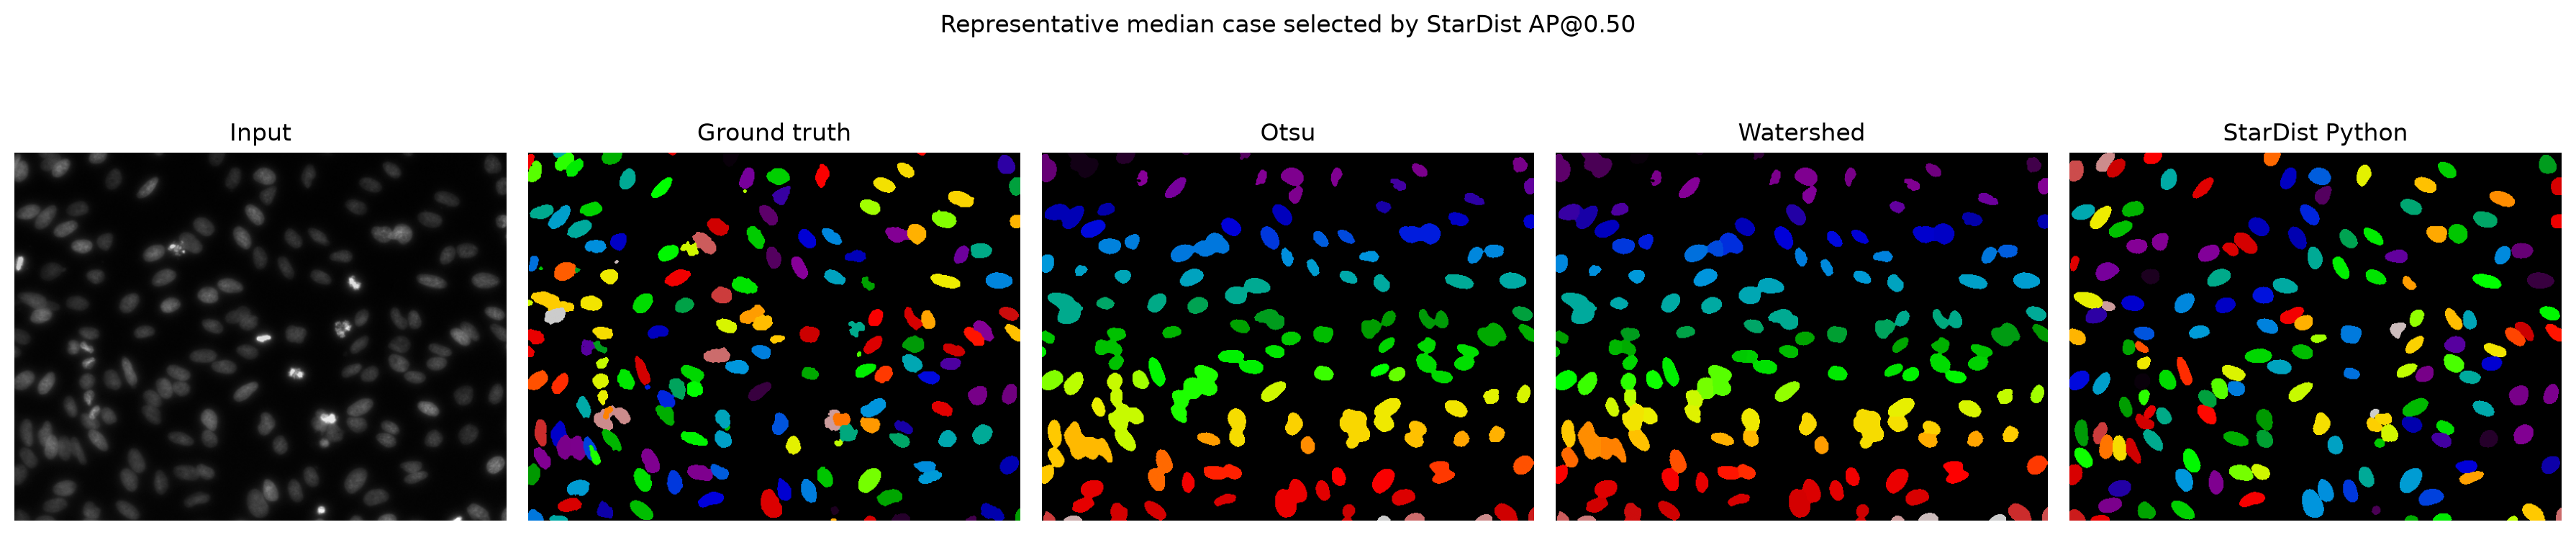
\includegraphics[width=\textwidth]{../results/dsb2018_benchmark/figures/qualitative_median.png}
\caption{Case trung vị theo AP@0.50 của StarDist trong 50 ảnh test. Màu biểu
diễn ID instance, không phải lớp semantic. Otsu gộp nhiều nhân tiếp xúc;
Watershed tách được một phần; StarDist bám theo instance ground truth sát hơn.}
\label{fig:qualitative-median}
\end{figure}

\begin{figure}[htbp]
\centering
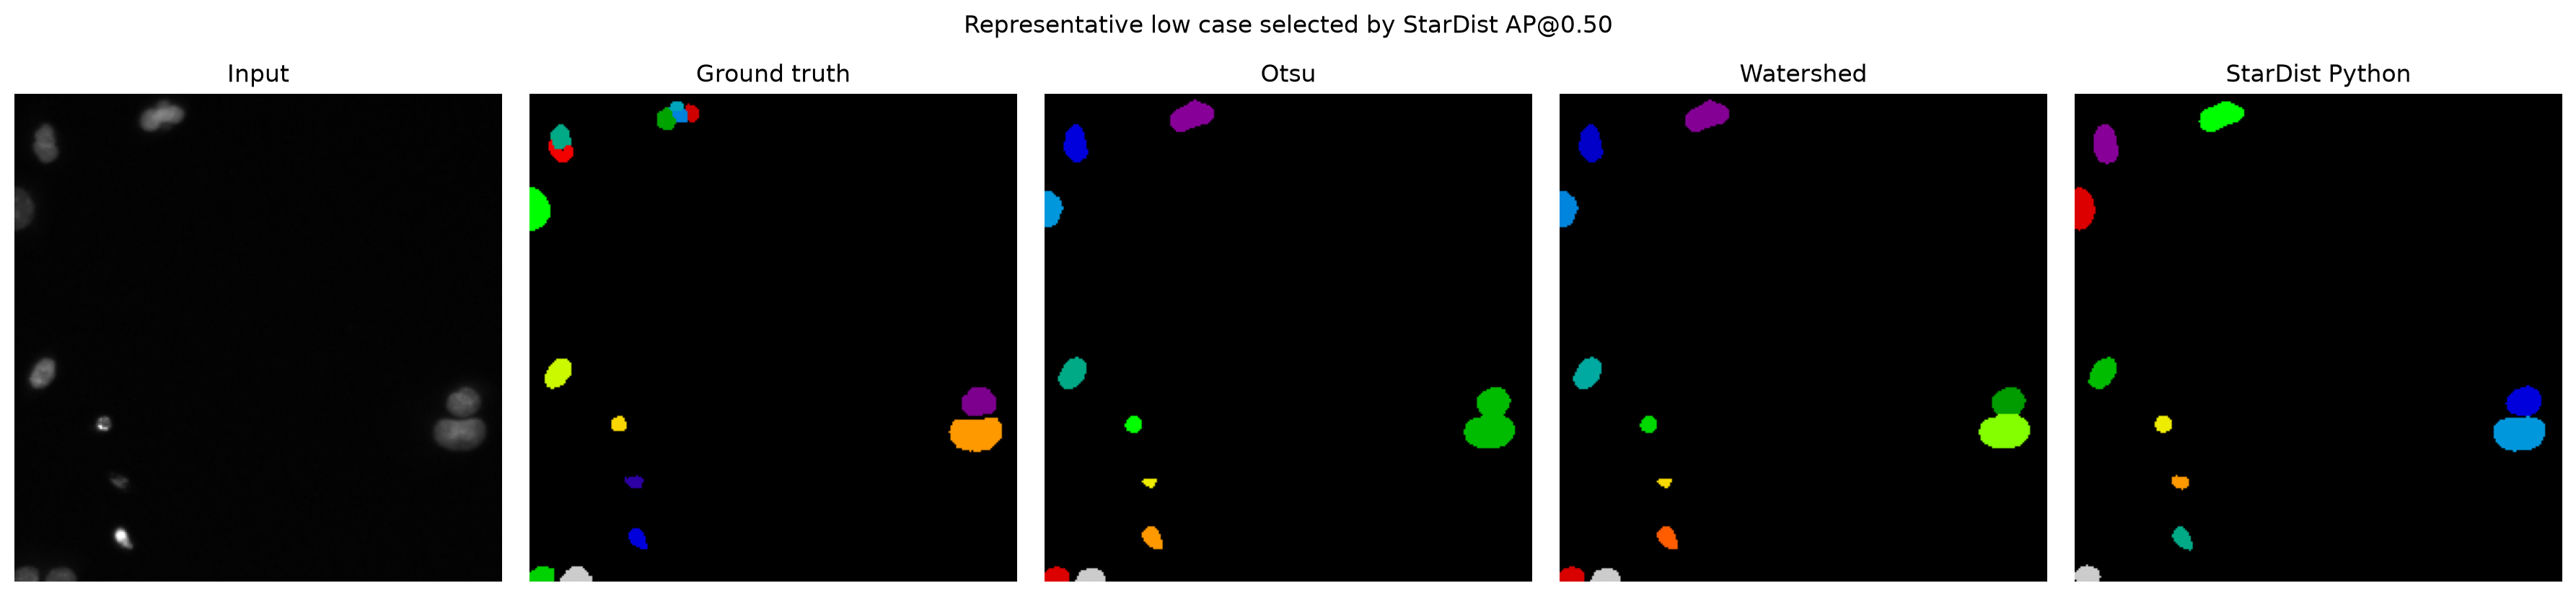
\includegraphics[width=\textwidth]{../results/dsb2018_benchmark/figures/qualitative_low.png}
\caption{Case có AP@0.50 thấp nhất của StarDist trong test split. Hình này
được báo cáo cùng case trung vị để tránh chỉ chọn ví dụ thuận lợi.}
\label{fig:qualitative-low}
\end{figure}

\begin{figure}[htbp]
\centering
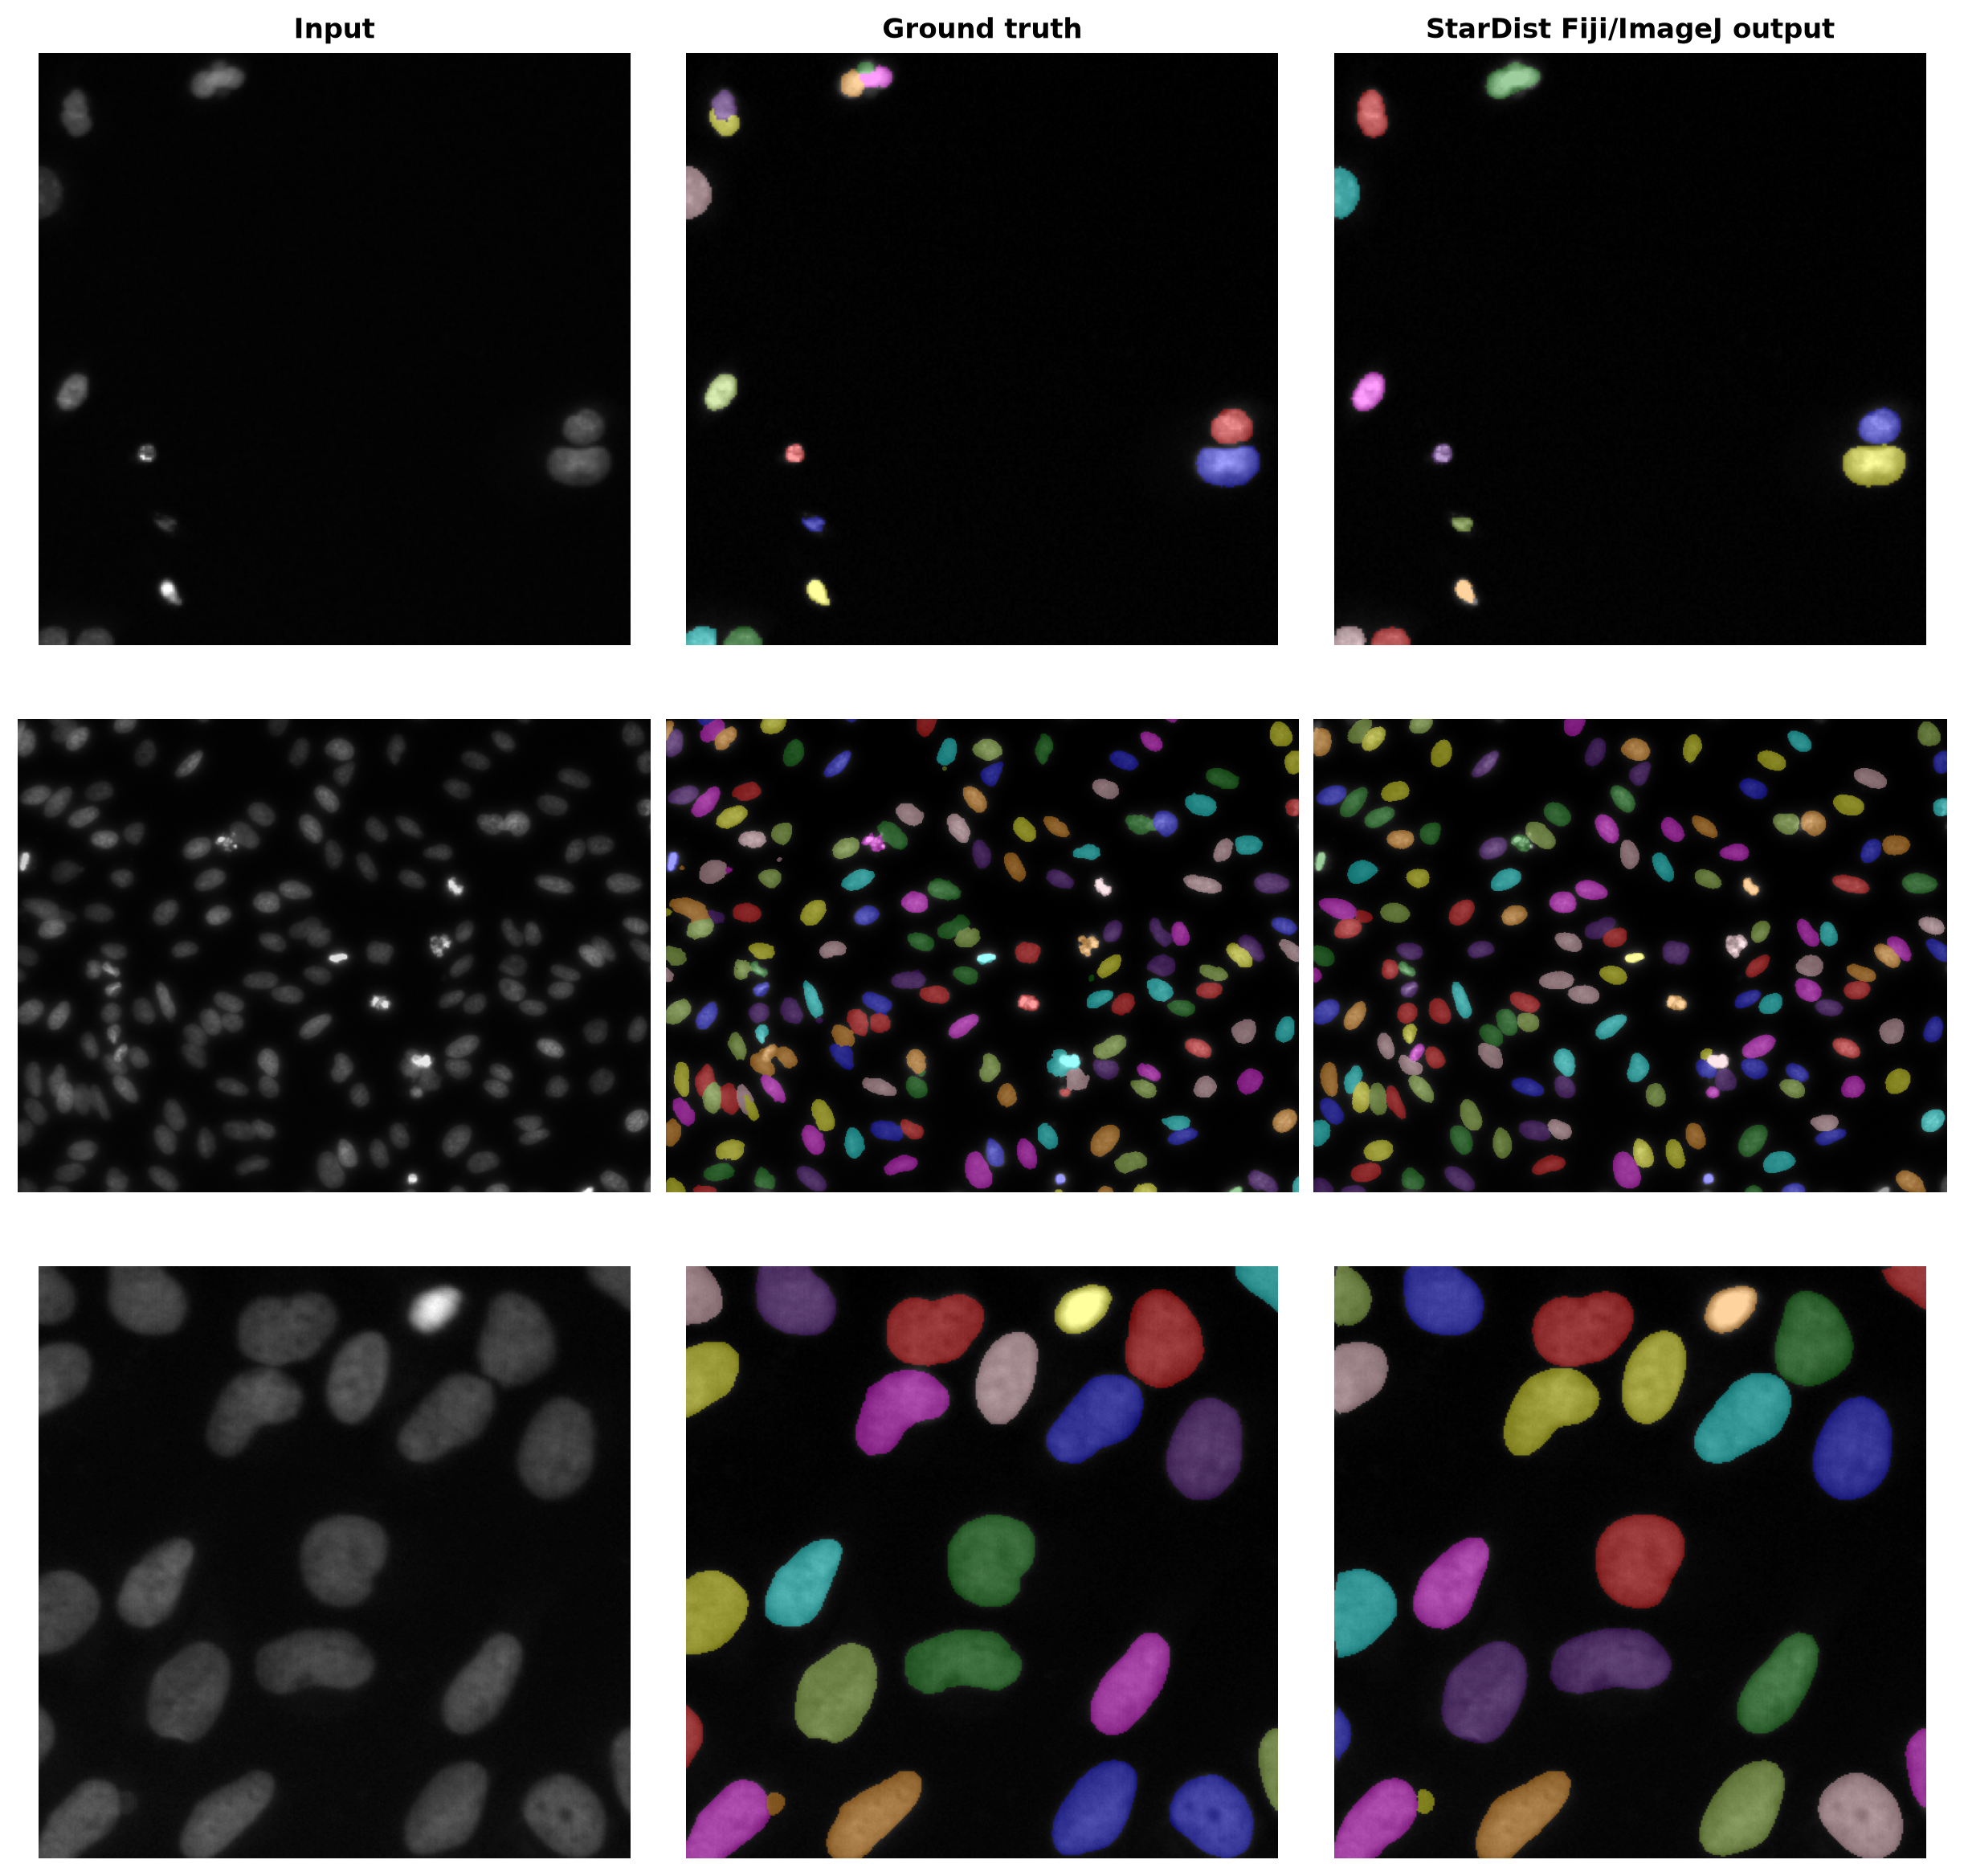
\includegraphics[width=.96\textwidth]{../results/fiji_reference/fiji_reference_panels.png}
\caption{Ba output Label Image thực tế của plugin StarDist Fiji/ImageJ: ca low,
median và high đã chọn trước, đặt cạnh input và ground truth. Mỗi màu là một ID
instance; figure được sinh trực tiếp từ TIFF plugin xuất.}
\label{fig:fiji-reference}
\end{figure}

\section{Cách đọc kết quả}
Trên 50 ảnh test, StarDist đạt AP@0.50 $0.853\pm0.120$ và PQ
$0.785\pm0.110$, cao hơn Watershed ($0.715\pm0.199$;
$0.677\pm0.166$) và Otsu ($0.643\pm0.238$; $0.627\pm0.208$). Dice foreground
của Otsu và Watershed gần $0.895$, nhưng AP instance thấp hơn: kết quả này
cho thấy Dice toàn foreground không đủ để đánh giá tách object. Watershed giảm
MAE đếm từ 14.06 xuống 6.94 so với Otsu; StarDist giảm tiếp còn 3.44. Ở
$\tau=0.90$, metric của cả ba giảm mạnh, phản ánh yêu cầu chính xác biên rất
nghiêm ngặt. StarDist chậm hơn baseline trên CPU (0.112 s/ảnh so với 0.024 s
Watershed), đổi lại tách instance tốt hơn trên benchmark này. Trên ba ca kiểm
chứng, plugin Fiji/ImageJ đạt AP@0.50 $0.801\pm0.244$, PQ $0.788\pm0.160$ và
Dice $0.950\pm0.017$; các TIFF/metric làm bằng chứng tương thích, không thay
thế benchmark $n=50$.

\section{Đe doạ tới tính hợp lệ}
Model pretrained có thể không phù hợp stain/optics của dữ liệu. Khác biệt Fiji
và Python có thể do version, normalization, tile hoặc NMS, không nhất thiết do
thuật toán. Dataset nhỏ dẫn tới SD lớn. Instance có hình không star-convex là
giới hạn cấu trúc; fine-tuning hoặc phương pháp khác cần được cân nhắc.

\chapter{Kết luận và hướng phát triển}
StarDist biến dự đoán pixel dày đặc thành tập polygon có định danh instance,
phù hợp với ảnh nhân tế bào đông đúc. Repo cung cấp pipeline kiểm chứng được
giữa Fiji/ImageJ và Python, baseline cổ điển, metric instance, label TIFF thực
tế và run log. Hướng phát triển là fine-tuning bằng annotation nội bộ, ablation
số tia, robustness với noise và đánh giá 3D.

\bibliographystyle{plainnat}
\bibliography{../references/references}
\appendix
\chapter{Phân công và checklist nộp bài}
\begin{longtable}{p{3cm}p{10cm}}
\toprule Thành viên & Công việc và artefact\\\midrule\endfirsthead
Thành viên 1 & Lý thuyết, mô hình toán, tài liệu: \texttt{docs/01\_ly\_thuyet\_stardist.md}.\\
Thành viên 2 & Package Python, test, CLI và \texttt{scripts/run\_experiment.py}.\\
Thành viên 3 & Fiji plugin, screenshot, macro, run log và label TIFF.\\
Thành viên 4 & Dataset, split, ground truth, bảng/biểu đồ và phân tích.\\
\bottomrule
\end{longtable}
Trước khi nộp LMS: thay tên/mã nhóm, chốt dataset và license, chạy test/lint,
điền bảng số liệu thật, thêm 4--6 hình minh hoạ/biểu đồ từ test set, xuất PDF
và kiểm tra số trang, cập nhật slide theo bảng cuối.

\chapter{Hướng dẫn tái lập đầy đủ}
\section{Cài môi trường và kiểm thử}
\begin{lstlisting}[language=Python]
python -m venv .venv
.venv\Scripts\python.exe -m pip install -e ".[dev,stardist]"
.venv\Scripts\python.exe -m pytest -q
.venv\Scripts\ruff.exe check src tests scripts
\end{lstlisting}
\section{Tạo lại kết quả và artefact}
\begin{lstlisting}[language=Python]
.venv\Scripts\python.exe scripts/run_real_demo.py
.venv\Scripts\python.exe scripts/build_fiji_workflow_evidence.py
\end{lstlisting}
Lệnh benchmark chính là `scripts/run\_dsb2018\_benchmark.py`; dataset TIFF đã
có trong repository, còn script chỉ tải archive DSB2018 và model
`2D\_versatile\_fluo` qua API chính thức khi chưa có cache. Nó lưu CSV, label
TIFF minh hoạ và figures. Lần chạy đã ghi trong báo cáo dùng CPU
Windows; TensorFlow native Windows từ 2.11 không dùng CUDA, nên benchmark GPU
phải ghi môi trường WSL2/Linux riêng. Phần ImageJ/Fiji tham chiếu đã lưu label
TIFF, figure, metric và run log trên ba ca. Trước nộp chỉ cần điền tên/MSSV/mã
nhóm rồi xuất PDF từ nguồn này.

\chapter{Mã nguồn cốt lõi}
\section{Matching và metric instance}
\lstinputlisting[language=Python,caption={`metrics.py`: IoU matrix, Hungarian matching và các metric.}]{../src/xla_gr03/metrics.py}
\section{Star-convex geometry reference}
\lstinputlisting[language=Python,caption={`geometry.py`: EDT, ray distance, polygon decode và NMS.}]{../src/xla_gr03/geometry.py}
\section{Script thí nghiệm chạy thật}
\lstinputlisting[language=Python,caption={`run\_real\_demo.py`: materialize sample, inference, evaluation và figure.}]{../scripts/run_real_demo.py}
\lstinputlisting[language=Python,caption={`run\_dsb2018\_benchmark.py`: validation, benchmark test split và tổng hợp kết quả.}]{../scripts/run_dsb2018_benchmark.py}
\section{Runner StarDist ImageJ/Fiji}
\lstinputlisting[language=Java,caption={\texttt{FijiStarDistRunner.java}: gọi command plugin, xuất Label Image TIFF và log runtime.}]{../fiji/scripts/FijiStarDistRunner.java}
\end{document}
